\documentclass[border=10pt]{standalone}
\usepackage{tikz}
\usetikzlibrary{automata, positioning, arrows.meta}

\begin{document}
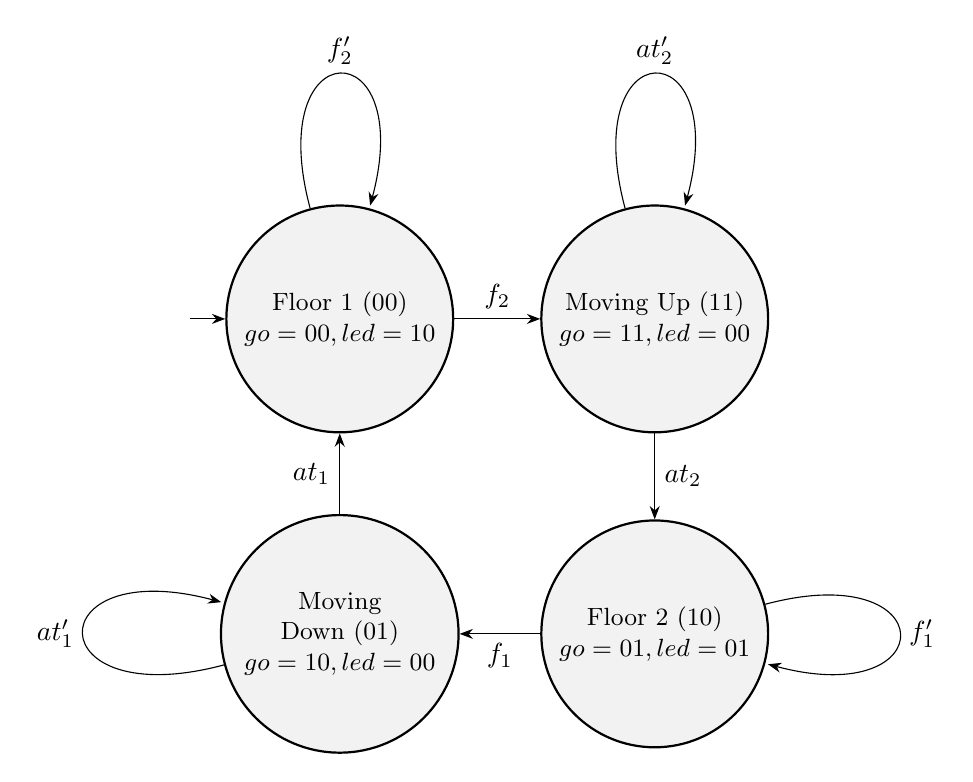
\begin{tikzpicture}[
    ->, >=Stealth, auto, node distance=4cm,
    every state/.style={thick, fill=gray!10, text width=2.5cm, align=center, font=\small},
    initial text=$ $
]

    % States
    % Outputs: go1, go0, led1, led2
    
    % State 00: Floor 1
    \node[state, initial] (s00) {Floor 1 (00) \\ $go=00, led=10$};
    
    % State 11: Moving Up
    \node[state, right of=s00] (s11) {Moving Up (11) \\ $go=11, led=00$};
    
    % State 10: Floor 2
    \node[state, below of=s11] (s10) {Floor 2 (10) \\ $go=01, led=01$};
    
    % State 01: Moving Down
    \node[state, left of=s10] (s01) {Moving Down (01) \\ $go=10, led=00$};

    % Transitions
    % From Floor 1
    \path (s00) edge[loop above] node {$f_2'$} (s00)
                edge node {$f_2$} (s11);
    
    % From Moving Up
    \path (s11) edge[loop above] node {$at_2'$} (s11)
                edge node {$at_2$} (s10);
    
    % From Floor 2
    \path (s10) edge[loop right] node {$f_1'$} (s10)
                edge node {$f_1$} (s01); % Bend left to go to s01 below
    
    % From Moving Down
    \path (s01) edge[loop left] node {$at_1'$} (s01)
                edge node {$at_1$} (s00);

\end{tikzpicture}
\end{document}
